\documentclass[14pt,a4paper]{extarticle}



\usepackage[utf8]{inputenc}
\usepackage[T2A]{fontenc}
\usepackage{amssymb,amsmath,mathrsfs,amsthm}
\usepackage[russian]{babel}
\usepackage{graphicx}
\usepackage[footnotesize]{caption2}
\usepackage{indentfirst}
\usepackage{multicol}
\usepackage{listings}
\usepackage{float}
\usepackage{url}

\usepackage{enumitem}

%\usepackage[ruled,section]{algorithm}
%\usepackage[noend]{algorithmic}
%\usepackage[all]{xy}
\usepackage{booktabs}
\usepackage{graphicx}
\usepackage[table,xcdraw]{xcolor}
\usepackage{tcolorbox}

%Библиотека для блок-схем
\usepackage{tikz}
\usetikzlibrary{shapes,arrows}

% Параметры страницы
\textheight=24cm
\textwidth=16cm
\oddsidemargin=5mm
\evensidemargin=-5mm
\marginparwidth=36pt
\topmargin=-1cm
\footnotesep=3ex
%\flushbottom
\raggedbottom
\tolerance 3000
% подавить эффект "висячих стpок"
\clubpenalty=10000
\widowpenalty=10000
%\renewcommand{\baselinestretch}{1.1}
\renewcommand{\baselinestretch}{1.5} %для печати с большим интервалом

\newcommand{\angstrom}{\mbox{\normalfont\AA}}

\newtheorem{definition}{Определение} % задаём выводимое слово (для определений)
\newtheorem{example}{Замечание} % задаём выводимое слово (для определений)
\newtheorem{theorem}{Теорема} % задаём выводимое слово (для определений)
\newtheorem{construction}{Конструкция} % задаём выводимое слово (для определений)

\DeclareMathOperator*{\sgn}{sgn}
\DeclareMathOperator*{\var}{var}   
\DeclareMathOperator*{\cov}{cov}
\DeclareMathOperator*{\law}{Law}

\newcommand{\1}{\mathbbm{1}} 
\newcommand{\R}{\mathbb{R}}
\newcommand{\N}{\mathbb{N}}
\newcommand{\Z}{\mathbb{Z}}
\renewcommand{\P}{\mathbb{P}}
\newcommand{\E}{\mathbb{E}}

\newcommand{\independent}{\perp\!\!\!\!\perp}


\newcommand\cA{{\cal A}}
\newcommand\cE{{\cal E}}
\newcommand\cC{{\cal C}}
\newcommand\cF{{\cal F}}
\newcommand\cG{{\cal G}}
\newcommand\cK{{\cal K}}
\newcommand\cL{{\cal L}}
\newcommand\cB{{\cal B}}
\newcommand\cN{{\cal N}}
\newcommand\cM{{\cal M}}
\newcommand\cX{{\cal X}}
\newcommand\cD{{\cal D}}
\newcommand\cR{{\cal R}}
\newcommand\cP{{\cal P}}
\newcommand\cQ{{\cal Q}}
\newcommand\cS{{\cal S}}
\newcommand\cT{{\cal T}}
\newcommand\cV{{\cal V}}
\newcommand\cZ{{\cal Z}}

\newcommand{\textProposition}    {Предложение}

\begin{document}

\begin{center}

{Всеволод Заостровский, 409 группа}\\
{\bfseries Отчёт по задаче "Приближение с помощью построения двумерного ряда Фурье".\\}
\vspace{1cm}

\end{center}

\section{Постановка задачи.}
Для функции $u(x) \in C^{\infty}[0, 1]$, удовлетворяющей краевым условиям:
\begin{align*}
    & u |_{\Omega} = 0,
\end{align*}
необходимо выписать двумерный тригонометрический ряд Фурье и сформулировать теорему сходимости. Затем, на сетке:

\begin{align*}
    & x_0 = \frac{-h_x}{2}, \; y_0 = \frac{-h_y}{2},\\
    & x_N = 1, \; y_N = 1, \\
    & h_x = h_y = h = \frac{1}{N - 0.5},
\end{align*}     

выписать двумерный дискретный тригонометрический ряд Фурье. \par
Найти дискретное скалярное произведение, сохраняющее ортогональность базисных функций. 
Нормировать базисные функции. 
\par
И, наконец, для некоторой тестовой функции из указанного класса численно найти порядок скодимости её дискретного ряда Фурье.

\section{Тригонометрический ряд Фурье.}
Функцию $u(x, y) \in C^{\infty}[0, 1]^2$ можно разложить в ряд Фурье, 
взяв синусы в качестве базисных функций:
\begin{equation*}
    u(x) = \sum_{m, n = 1}^{\infty} c_{mn} \sin {\pi m x} \sin {\pi n y}.
\end{equation*}
\par
Перейдём к рассмотрению конечного числа узлов. Выпишем условия на сетку:
\begin{align*}
    & u_{ij} := u(x_i, y_j), \; h = \frac{1}{N - 0.5}, \; x_i = y_i := \frac{-h}{2} + i h \\
    & u_{ij} = \sum_{c_{mn}} c_{mn} \phi_i^m \phi_j^n, \\
    & \phi_i^m := \sin{\pi m (\frac{-h_x}{2} + i h_x)} = \sin{\pi m (\frac{-h}{2} + i h)} \\
    & \phi_j^n := \sin{\pi n (\frac{-h_y}{2} + j h_y)} = \sin{\pi n (\frac{-h}{2} + j h)} \\
    & \phi^m := (\phi_1^m ... \phi_{N-1}^m).
\end{align*} 
Убедимся, что указанные функции ортогональны относительно скалярного произведения 
${(\phi^k, \phi^j) = \sum_{m = 1}^{N - 1}\phi_m^k \phi_m^j h}$:

\begin{align*}
    & (\phi^k, \phi^j) = \sum_{m = 1}^{N - 1} \phi_m^k \phi_m^j h 
    = \sum_{m = 1}^{N - 1} \sin{\pi k (\frac{-h}{2} + m h)} \sin{\pi j (\frac{-h}{2} + m h)} h \\ 
    & = \frac{1}{2} \sum_{m = 1}^{N - 1} [ \cos{(\pi h (m - \frac{1}{2})(k - j))} - \cos{(\pi h (m - \frac{1}{2})(k + j))} ] h.
\end{align*}

Заметим, что при $\alpha \neq 0$ справедливо:
\begin{align*}
    & \sum_{m = 1}^{N - 1} \cos(\alpha m - \frac{\alpha}{2}) = Re\sum_{m = 1}^{N - 1} e^{i (\alpha m - \frac{\alpha}{2})} 
     = Re \frac{e^{\frac{i \alpha}{2}(e^{i \alpha (N - 1)} - 1)}}{e^{i \alpha - 1}} 
     = \frac{Im [-1 + e^{i (N - 1) \alpha}]}{2 \sin(\alpha/2)} \\
    & = \frac{\sin{(N - 1) \alpha}}{2 \sin(\alpha/2)}.
\end{align*}

Отсюда при $k \neq j$:

\begin{align*}
    & (\phi^k, \phi^j) 
    = \frac{1}{2} \sum_{m = 1}^{N - 1} [ \cos{(\pi h (m - \frac{1}{2})(k - j))} - \cos{(\pi h (m - \frac{1}{2})(k + j))} ] h \\
    & = h \left[ \frac{\sin{(N - 1) \pi h (k - j)}}{4 \sin(\pi h (k - j)/2)} - \frac{\sin{(N - 1) \pi h (k + j)}}{4 \sin(\pi h (k + j)/2)} \right] \\
    & = h \left[ \frac{\sin(\pi (k - j) - \pi h (k - j))}{4 \sin(\pi h (k - j)/2)}
        - \frac{\sin(\pi (k + j) - \pi h (k + j))}{4 \sin(\pi h (k + j)/2)}\right] \\
    & = h \left[ \frac{(-1)^{k-j}\sin(\pi h (k - j))}{4 \sin(\pi h (k - j)/2)}
    - \frac{(-1)^{k+j}\sin(\pi h (k + j))}{4 \sin(\pi h (k + j)/2)}\right] \\
    & = \frac{h}{2} [(-1)^{k-j}\sin(\pi h (k - j)/2) - (-1)^{k+j}\sin(\pi h (k + j)/2)] = 0.
\end{align*}

В ином случае, 
\begin{align*}
    & (\phi^k, \phi^k) 
    = \frac{1}{2} \sum_{m = 1}^{N - 1} [ \cos{(\pi h (m - \frac{1}{2})(k - k))} - \cos{(\pi h (m - \frac{1}{2})(k + k))} ] h \\
    & = h \left[ \frac{N - 1}{2} - \frac{\sin{2 (N - 1) \pi h k}}{4 \sin(\pi h k)} \right] 
    = \frac{2 N - 1}{4} \frac{2}{2 N - 1} = \frac{1}{2}.
\end{align*}

Отсюда, очевидно, система функций $\psi_{ij}^{mn} := \phi_i^m \phi_j^n $. \par
Искать коэффициенты будем по следующему алгоритму: 
\begin{enumerate}
    \item Вычислим матрицу $u_{ij}$.
    \item Разложим $u_{ij}$ в одномерный ряд Фурье:
        \begin{equation*}
            u_{ij} = \sum _{m = 1}^{N - 1} \phi_i^m d_m^j.
        \end{equation*}
        Полученные коэффициенты запишем в новую матрицу.
    \item По вектору $d_m^j$ восстановим коэффициенты $c_{mn}$ посредством ещё одного разложения в ряд:
        \begin{equation*}
            d_m^j = \sum _{n = 1}^{N - 1} c_{mn} \phi_j^n.
        \end{equation*}
\end{enumerate}


\section{Тесты}
\subsection{Тест 1}
Рассматривалась функция:
\begin{lstlisting}[language=c]
    double u(double x)
{
    return x * (1 - x) * y * (1 - y);
}
    \end{lstlisting}

    \begin{figure}
        \centering
        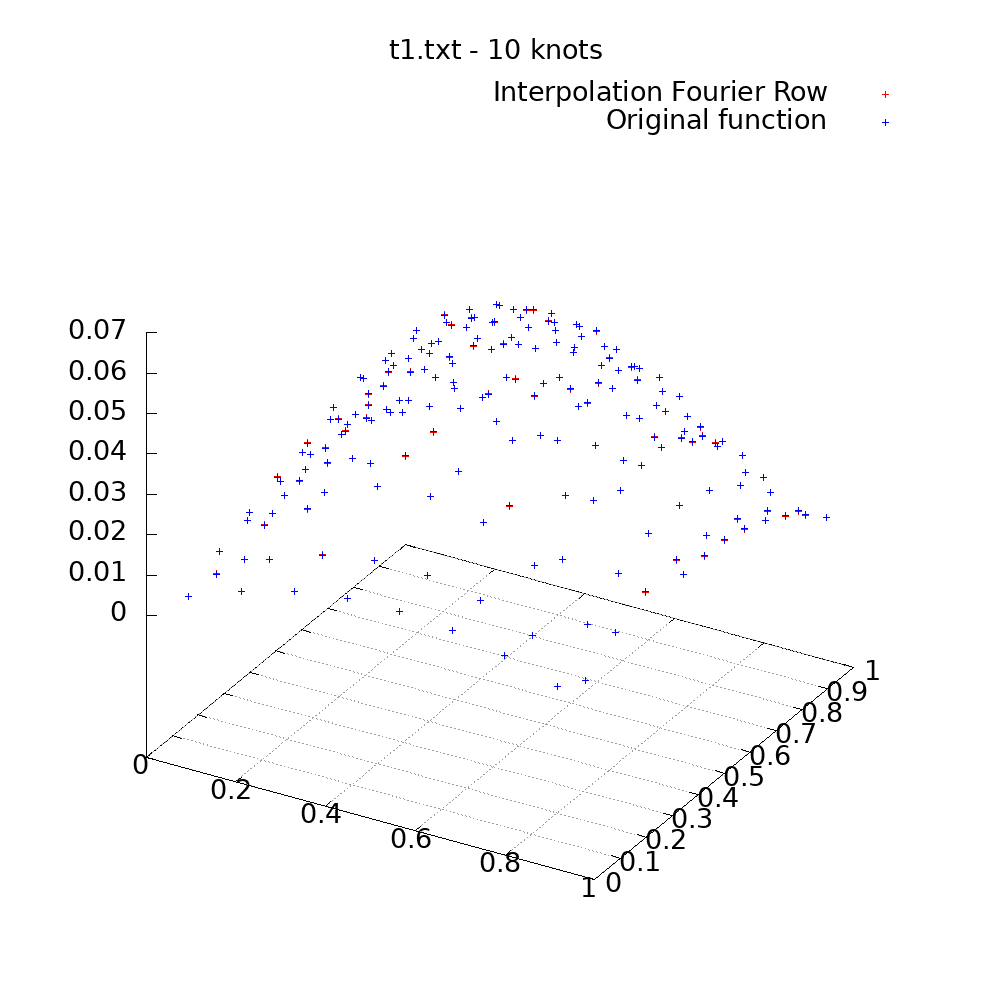
\includegraphics[scale=0.5]{Images/t1.txt.png}
        \caption{Результаты теста функции $x * (1 - x) * y * (1 - y)$.}
    \end{figure}

\begin{figure}
    \centering
    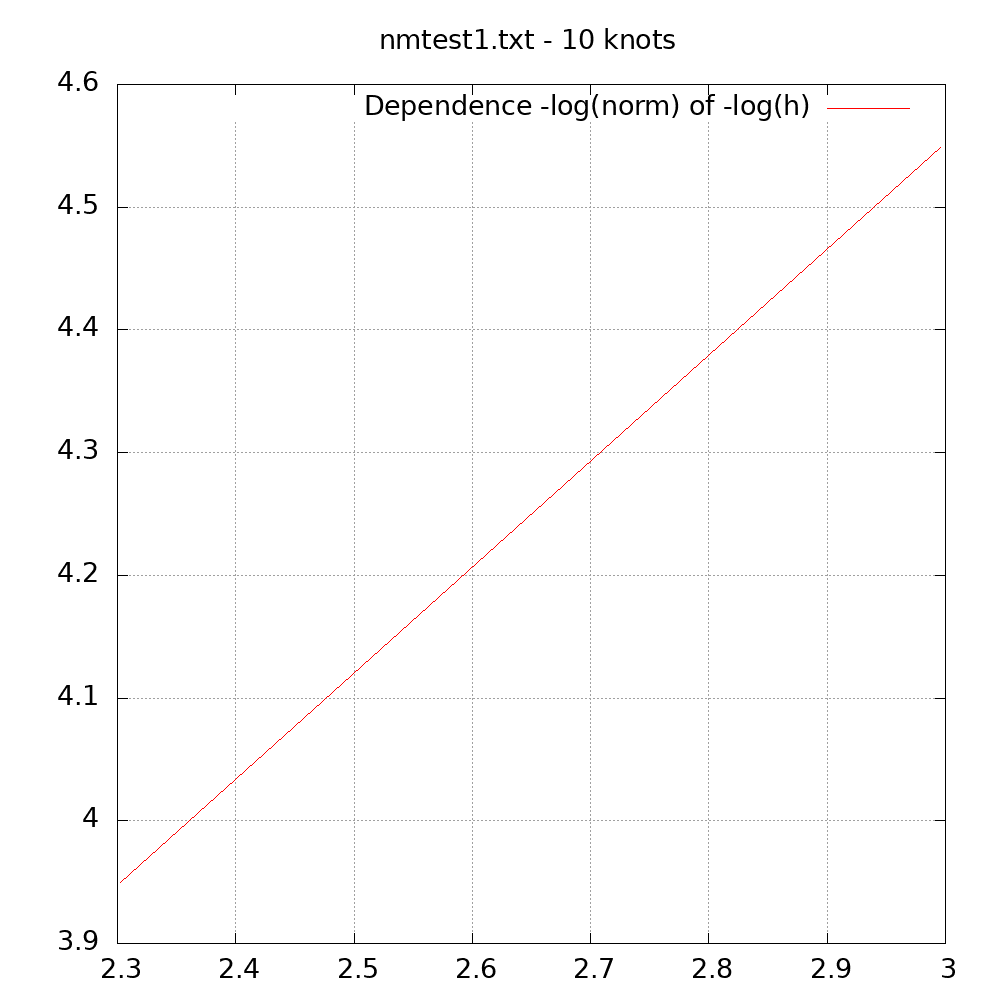
\includegraphics[scale=0.5]{Images/nmtest1.txt.png}
    \caption{Результаты теста функции $x * (1 - x) * y * (1 - y)$.}
\end{figure}


\subsection{Тест 2}
Рассматривалась функция:
\begin{lstlisting}[language=c]
    double u(double x, double y)
{
    return x * (1 - x) * y * (1 - y) * cos(x * x) * cos(y * y);
}
    \end{lstlisting}

    \begin{figure}
        \centering
        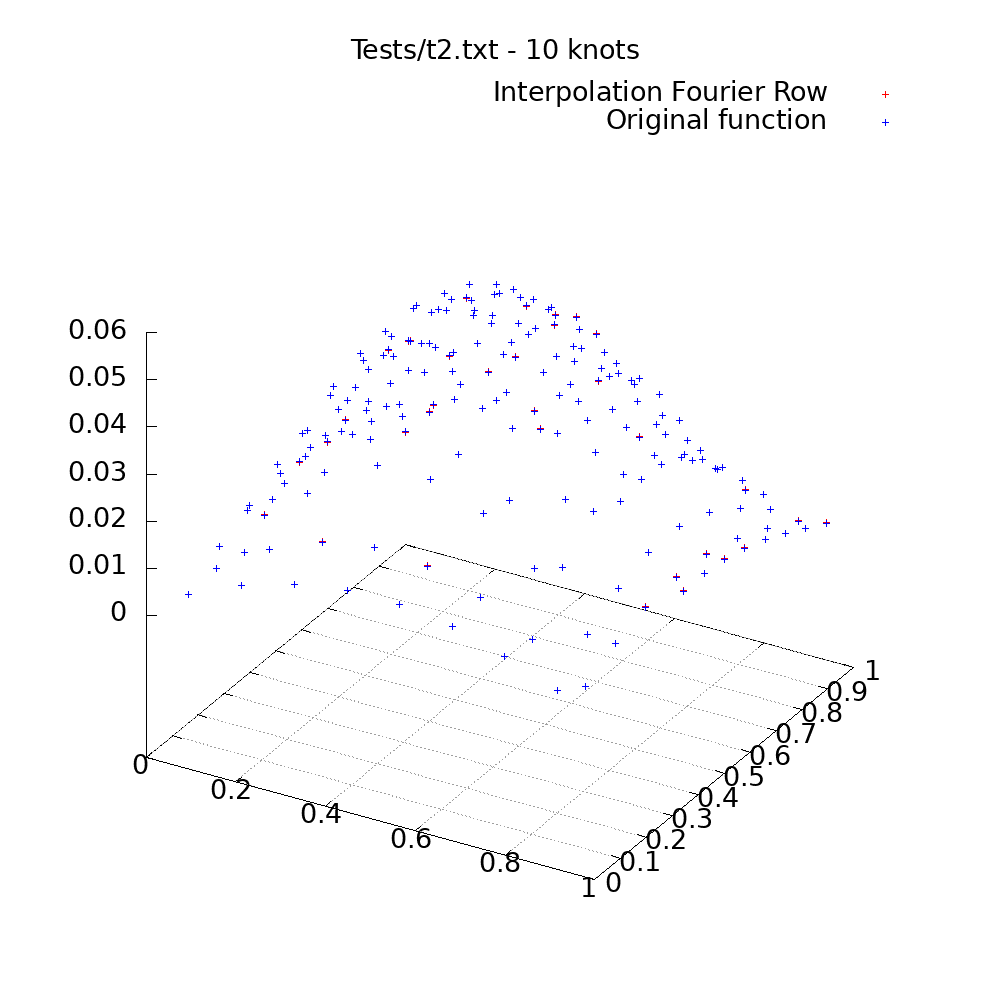
\includegraphics[scale=0.5]{Images/t2.txt.png}
        \caption{Результаты теста функции $x * (1 - x) * y * (1 - y) * cos(x * x) * cos(y * y)$.}
    \end{figure}

\begin{figure}
    \centering
    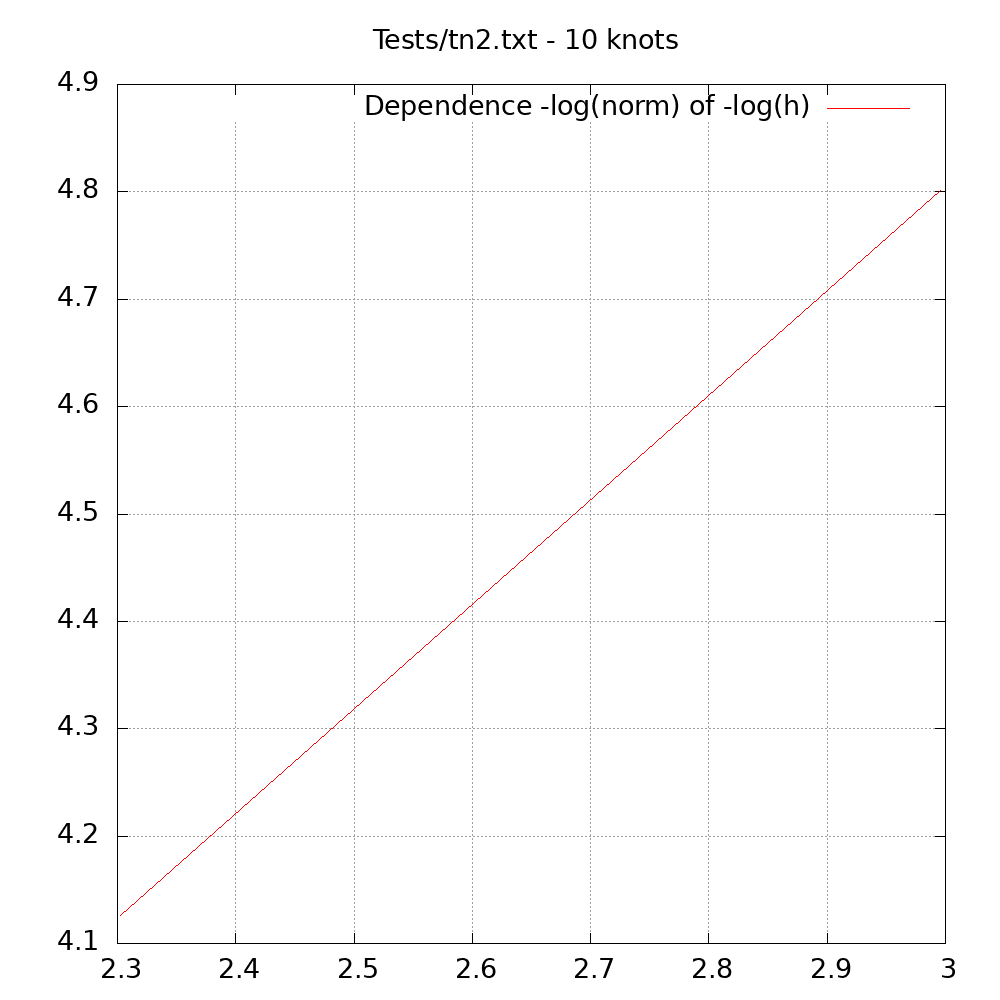
\includegraphics[scale=0.5]{Images/tn2.txt.png}
    \caption{Результаты теста функции $x * (1 - x) * y * (1 - y) * cos(x * x) * cos(y * y)$.}
\end{figure}



\end{document}